\chapter{\sf Numerical Methods}\label{ch:numerics}

This chapter begins with the derivation of the time-stepping equation used to simulate the PFC model's dynamics. Then, this equation's discretization and implementation are described. Following that, the procedure for calculating nucleation rates is presented. Finally, numerical tools for analyzing the early stages of grain formation, including the form of critical nuclei, are developed.

%%%%%%%%%%%%%%%%%%%%%%%%%%%%%%%%%%%%%%%%%%%%%%%%%%%%%%%%%%%%%%%%%%%%%%%%%%%%%%%%%%%%
\section{Semi-implicit Fourier space method for solving PFC dynamics}\label{sec:num_pfc}

We obtain the time-stepping equations for the PFC model's dynamics using a semi-implicit Fourier space method \cite{provatas_PFC}. Begin by rewriting equation \ref{eq:pfc_dynamics_dimensionless_final} as
%%
\begin{equation}\label{eq:num_rewritten_pfc}
\frac{\partial n}{\partial t} = Ln + \nabla^2 N(n) + R
\end{equation}
%%
where $L=\nabla^2(B^l +B^x (2\nabla^2+\nabla^4))$, $N=-tn^2+vn^3$, and $R=\nabla \cdot \vec\xi$. We have taken $\Gamma=1$ for all our simulations. We assume the nonlinear term $N(n)$ and the noise term $R$ are calculated in real space at each time step. We take the Fourier transform of \ref{eq:num_rewritten_pfc}, giving
%%
\begin{equation}\label{eq:num_rewritten_pfc_fourier}
\frac{\partial \hat{n}_k}{\partial t} = \hat{L}_k \hat{n}_k - k^2 \hat{N}_k + \hat{R}_k
\end{equation}
%%
where $\hat{L}_k = - k^2(B^l +B^x (-2k^2+k^4))$, $\hat{N}_k$ and $\hat{R}_k$ are the respective transforms of $N$ and $R$, and $k^2=(k_x^2+k_y^2)$ is the wavevector's squared magnitude.

Approximating equation \ref{eq:num_rewritten_pfc_fourier} to be a first-order ordinary differential equation in $\hat{n}_k$, and defining $\hat{D}_k(t)=- k^2 \hat{N}_k + \hat{R}_k$, we write its solution as
%%
\begin{equation}\label{eq:num_pfcfourier_odesol}
\hat{n}_k(t)=\hat{n}_k(0) + e^{\hat{L}_k t}\int_0^t e^{-\hat{L}_k s}\hat{D}_k(s) ds
\end{equation}
%%
which can be rearranged at shifted time $t+\Delta t$ to give
%%
\begin{equation}\label{eq:num_pfcfourier_odesol_timeshift}
\begin{split}
\hat{n}_k(t+\Delta t)&=\hat{n}_k(0) + e^{\hat{L}_k (t+\Delta t)}\int_0^{t+\Delta t} e^{-\hat{L}_k s}\hat{D}_k(s) ds
\\&=\hat{n}_k(0) + e^{\hat{L}_k (t+\Delta t)} \left(\int_0^{t}+\int_t^{t+\Delta t} \right) e^{-\hat{L}_k s}\hat{D}_k(s) ds
\\&=e^{\hat{L}_k \Delta t}\hat{n}_k(t) + e^{\hat{L}_k (t+\Delta t)} \int_t^{t+\Delta t} e^{-\hat{L}_k s}\hat{D}_k(s) ds
\end{split}
\end{equation}
%%
The final approximation is to assume that $\hat{D}_k(t)$ varies much more slowly with $t$ than $e^{-\hat{L}_k t}$, leading us to write
%%
\begin{equation}
\int_t^{t+\Delta t} e^{-\hat{L}_k s}\hat{D}_k(s) ds \approx \hat{D}_k(t)\int_t^{t+\Delta t} e^{-\hat{L}_k s} ds = \frac{-e^{-\hat{L}_k t}(e^{-\hat{L}_k \Delta t}-1)}{\hat{L}_k}  \hat{D}_k(t)
\end{equation}
%%
which is then plugged into equation \ref{eq:num_pfcfourier_odesol_timeshift} to give the time-stepping equation
%%
\begin{equation}\label{eq:num_pfc_final}
\hat{n}_k(t+\Delta t)\approx e^{\hat{L}_k \Delta t}\hat{n}_k(t) +\frac{e^{\hat{L}_k \Delta t}-1}{\hat{L}_k} ( - k^2 \hat{N}_k + \hat{R}_k )
\end{equation}
%%

The advantage of using this semi-implicit method over a simpler method such as Euler time-stepping is that the semi-implicit method is stable for larger time steps $\Delta t$, allowing more efficient computation for the simulations.

%%%%%%%%%%%%%%%%%%%%%%%%%%%%%%%%%%%%%%%%%%%%%%%%%%%%%%%%%%%%%%%%%%%%%%%%%%%%%%%%%%%%
\section{Implementation of the time-stepping equation}\label{sec:num_discret}

Equation \ref{eq:num_pfc_final} is numerically calculated on a grid with spacing $dx=a/8$, where $a$ is the dimensionless lattice constant, and with time spacing $dt=1$. The size of the grid is $L \times L$, with $L$ a power of 2 chosen depending on the specific simulation run's goal (see following sections). Periodic boundary conditions are used on this grid.

The procedure to advance the simulation by one time step is as follows:
\begin{enumerate}
\item Generate the noise term $R=\nabla \cdot \vec\xi$ in real space. To do this, first generate two discrete fields $X$ and $Y$, corresponding to the two component fields of $\vec\xi$, whose points are uncorrelated random variables of Gaussian distribution, zero mean, and standard deviation $\sigma = N_a/\sqrt[]{dx^2dt}$. Then the discrete $R$ is given by
%%
\begin{equation}
R_{ij}=(X_{ij}-X_{i-1j}+Y_{ij}-Y_{ij-1})/dx
\end{equation}
%%
\item Calculate the nonlinear term $N=-tn^2+vn^3$ in real space.
\item Apply the well-known Fast Fourier Transform (FFT) algorithm on $N$ and $R$ to obtain $\hat{N}_k$ and $\hat{R}_k$.
\item Apply the noise spectrum cut-off discussed in section \ref{sec:pfc_dynamics}, by setting the grid points of the discrete $\hat{N}_k$ corresponding to wavenumbers with $k>2\pi/a$ to zero.
\item Calculate the new Fourier transformed discrete dimensionless density field $\hat{n}_k$ in Fourier space using equation \ref{eq:num_pfc_final}.
\item Apply the inverse FFT algorithm on $\hat{n}_k$ to obtain the real-space $n$, to be used in calculating the nonlinear term in the next time step.
\end{enumerate}

The code for this procedure is implemented in MATLAB, using that software's Parallel Computing Toolbox to enable computation on a Graphics Processing Unit (GPU). Early prototypes of the code where implemented in the C programming language, using the CUDA libraries to run the computationally-intensive subsets of the code on a GPU. Although the C version of the code showed speeds around $3\times$ that of the MATLAB code, the ease of implementation of analysis tools in MATLAB led to the eventual switch. The code ran on a laptop equipped with a NVIDIA GeForce GTX 960M GPU device.


%%%%%%%%%%%%%%%%%%%%%%%%%%%%%%%%%%%%%%%%%%%%%%%%%%%%%%%%%%%%%%%%%%%%%%%%%%%%%%%%%%%%
\section{Simulations for calculation of post-critical nuclei densities}\label{sec:num_rates}

For a given set of parameters $B^l$, $B^x$, $n_o$, and $N_a$, obtaining the PFC model's time-evolving post-critical nuclei densities involves averaging the results of a large number of simulation runs. Each simulation run has grid size given by $L=1024$, and as initial condition a system full of liquid, $n(\vec{x})=n_o$.

Every $N_{out}=50$ time steps (defined as one `output step') in a given run, the local maxima of the discretized field $n$ are obtained by comparing each grid point with its 8 neighbors. The maxima that surpass a chosen threshold are considered peaks of the periodic function $n$, and their positions are stored. The threshold is taken to be half the maximum deviation of the periodic function from the liquid average density, i.e. $n_o + 0.75\phi_s$ where $\phi_s$ was obtained in equation \ref{eq:freeEnergy_minima}. For what follows, these peaks are assumed to be the position of atoms in the crystal lattice of formed solid regions.

Each run is set to last until 90\% of the maximum possible number of peaks have formed. Assuming the chosen parameters place the system below the phase diagram's solidus, and knowing that the formed lattice structure is triangular with lattice constant $a$, we can calculate the maximum number $M_p$ of peaks that can appear in the simulation by dividing the total simulation area by the area of the lattice's unit cell, giving
%%
\begin{equation}
M_p = \frac{(dx\,L)^2}{(\sqrt[]{3}/2)a^2}
\end{equation}
%%

Once all runs are complete, the obtained peaks are used to count the number of nucleation events that occurred. To do so, the peaks must be grouped into separate clusters, representing individual crystal grains that have formed and possibly grown. The clusters must remain distinguishable even after their growth leads to impingement of their grain boundaries. 

\begin{figure}[!ht]
    \centering
\begin{tabular}{cccc}
\subfloat[]
{
    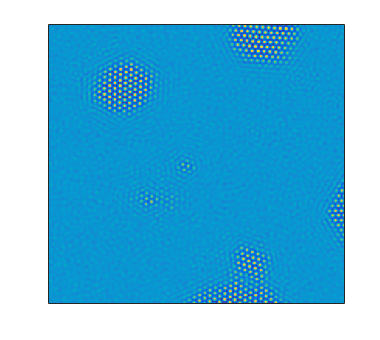
\includegraphics[width=0.5\textwidth]{fig_num/clustEx_1b}
}
&\subfloat[]
{
    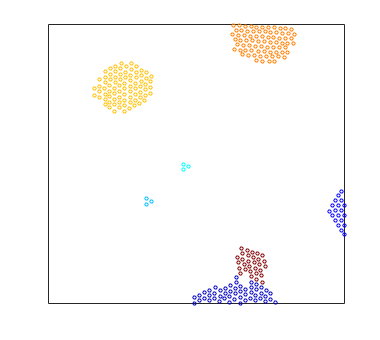
\includegraphics[width=0.5\textwidth]{fig_num/clustEx_1a}
}\\
\subfloat[]
{
    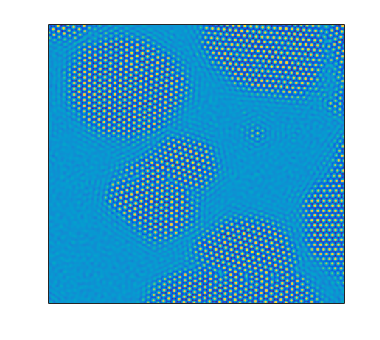
\includegraphics[width=0.5\textwidth]{fig_num/clustEx_2b}
}
&\subfloat[]
{
    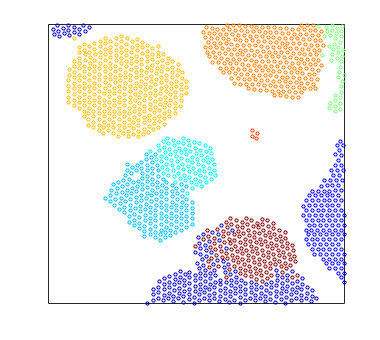
\includegraphics[width=0.5\textwidth]{fig_num/clustEx_2a}
}
\end{tabular}
    \caption{(a) and (c) show two snapshots of the density field $n$ in a small area of a simulation run, ordered by time. (b) and (d) show the corresponding detected peaks, grouped into clusters shown by color.}\label{fig:num_clustexample}
\end{figure}

Here we state our method for grouping peaks into clusters. Let $P(t)$ be the set of all peaks found at time $t$ in a specific run, and let $d(p_1,p_2)$ be the function which gives the distance between two peaks $p_1 , p_2 \in P(t)$. Let $C(t)$ be the set of all clusters at time $t$, with each of its elements consisting of a subset of $P(t)$ representing the peaks in a specific cluster. The procedure to determine $C(t)$ at a time $t$, given the set $P(t)$, is as follows: 
\begin{enumerate}
\item Set $C(t)=C(t-N_{out}dt)$, where $t-N_{out}dt$ is the time of the previous output step. If this is the first output step, set $C(t)$ to be the empty set.
\item For every $c \in C(t)$, remove peaks $p\in c$ where $p \notin P(t)$. This removes peaks that have vanished since the previous output step.
\item For every $p_1\in P(t)$ where $p_1$ belongs to no cluster in $C(t)$, check if $d(p_1,p_2)<3a$ for any peak $p_2\in c$ for any $c\in C(t)$. If so, add $p_1$ to cluster $c$. This adds peaks which appeared due to a previously-present growing cluster to that cluster. The distance value $3a$ was chosen to allow leeway for peaks appearing further than the lattice constant $a$ before merging fully with the cluster that generated them. This also accounts for some possible heterogeneous nucleation events, which we do not wish to count as separate clusters that would skew the homogeneous nucleation rate calculation. Repeat this step of the procedure until no $p_1$ is left that satisfies the distance requirement.
\item If there remains any $p\in P(t)$ that belong to no cluster of $C(t)$, choose one of these $p$ at random. Define a new cluster in $C(t)$ consisting of only that peak. Then return to step 3 of this procedure. This ensures that eventually all peaks are sorted into a cluster.
\end{enumerate}


Figure \ref{fig:num_clustexample} shows two zoomed-in snapshots of a simulation run, along with corresponding plots of the detected peaks grouped into clusters using the above method. Note that the method does not always perfectly separate impinging clusters at their lattice boundaries. This is not an issue as we are interested in the number of such distinguishable clusters, rather than their exact final size.

In our simulation runs, we observed that any cluster consisting of 3 or more detected peaks tended to keep growing far more often than shrinking. As such, we assume that clusters with 3 or more peaks represent post-critical nuclei. Note that this assumption does not imply that the exactly critical nuclei must have 3 atoms, as the detected peaks only account for peaks above the threshold defined previously, without accounting for other factors in the form of crystal grains that determines whether they are critical nuclei. The set of clusters $C(t)$ is then used to obtain the number of such nuclei in one run as a function of time. Summing this number over all runs that use the same set of parameters, and dividing by the total simulation area of all these runs, yields our value for the number of post-critical nuclei per area as a function of time. This value can then be compared to CNT's prediction for $I^*(t)$ as mentioned in section \ref{sec:nuc_cnt_pfc}.




%%%%%%%%%%%%%%%%%%%%%%%%%%%%%%%%%%%%%%%%%%%%%%%%%%%%%%%%%%%%%%%%%%%%%%%%%%%%%%%%%%%%
\section{Wave mode analysis}\label{sec:num_wave}

As described in section \ref{sec:pfc_1mode}, the PFC model's density field $n$ can be expanded in terms of three wave modes, corresponding to the lowest order reciprocal lattice vectors of the triangular lattice. In the solid phase, these three wave modes would have equal amplitude. However, it is unclear whether the amplitude of all three of these wave modes must fluctuate to a nonzero value simultaneously for a stable solid grain to form from a liquid phase, or whether the wave modes can separately appear and build up to a stable nucleus over time. To better understand this early stage of grain formation in terms of the wave modes, we here develop a method to quantify the relative amplitudes of the present modes at the positions and times where grains appear in the simulations. Our method expands on work by Singer and Singer \cite{singer06}, where a method is developed to visualize the orientation of crystal grains in a fully solidified system.

We construct a `test wavelet', whose density field is given by one of the solid phase's wave modes multiplied to a Gaussian envelope, written as
%%
\begin{equation}
n_{w}(\vec{x}) = Ne^{-|\vec{x}|^2/2\sigma^2}\cos(2\pi \vec{q}\cdot\vec{x})
\end{equation}
%%
where $\vec{q}$ is one of the lowest order reciprocal lattice vectors, $N$ is a normalization constant that ensures the integral over the area of the wavelet is unity, and the standard deviation of the Gaussian is chosen to be $\sigma=0.8a$ for $a$ the lattice constant. Figure \ref{fig:num_testWavelet} shows this test wavelet.

\begin{figure}[h]
\centering
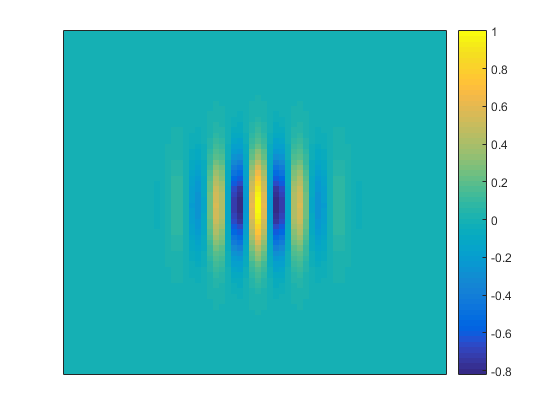
\includegraphics[width=0.5\textwidth]{fig_num/testWavelet.png}
\caption{The test wavelet for $\vec{q}$ chosen to be along the horizontal direction. The wavelet is shown unnormalized for clarity.}\label{fig:num_testWavelet}
\end{figure}

We convolve the test wavelet with the density field $n$ obtained from a simulation run, at a specific time $t$. This convolution enhances features of $n$ that exhibit the same structure as the wavelet. We then also apply a local averaging filter to smooth the field. The resulting filtered field's value provides at each spatial location a relative estimate of the amplitude of the wave mode corresponding to the wavelet's $\vec{q}$. By rotating the wavelet before applying this filtering process, the presence of a different wave mode can be examined. Figure \ref{fig:num_convtest} shows a snapshot of a simulation run, as well as the result of applying the filters on it for various rotations of the test wavelet. This filtering process can be applied every few time steps of a nucleation-rate simulation, for a range of rotation angles, to obtain the relative amplitude growth of wave modes at points where nucleation occurs.

\begin{figure}[!ht]
    \centering
\begin{tabular}{cccc}
\subfloat[]
{
    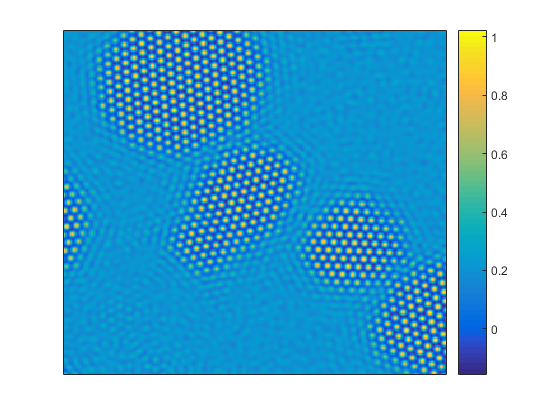
\includegraphics[width=0.5\textwidth]{fig_num/convtest1}
}
&\subfloat[]
{
    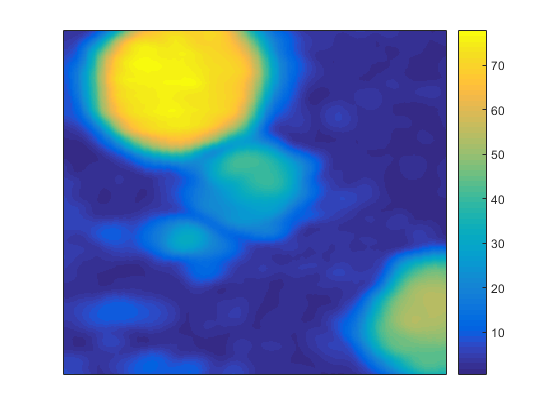
\includegraphics[width=0.5\textwidth]{fig_num/convtest2}
}\\
\subfloat[]
{
    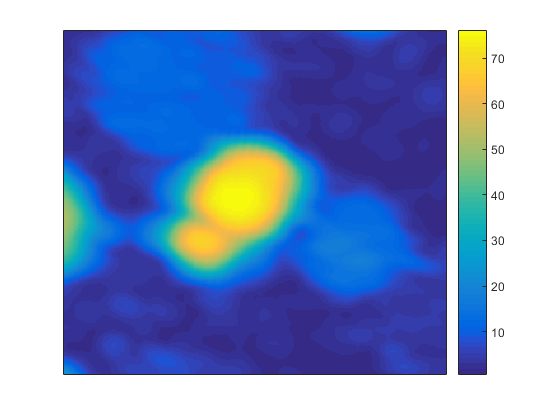
\includegraphics[width=0.5\textwidth]{fig_num/convtest3}
}
&\subfloat[]
{
    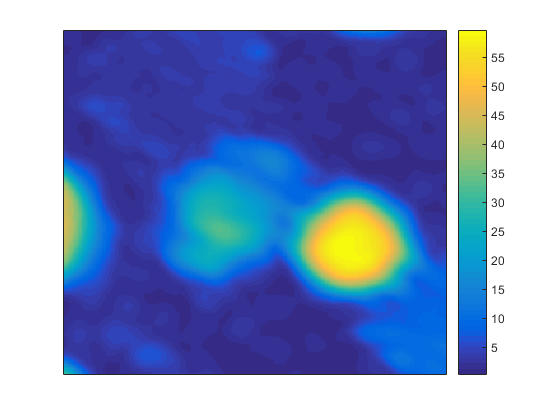
\includegraphics[width=0.5\textwidth]{fig_num/convtest4}
}
\end{tabular}
    \caption{(a) The density field $n$ at a specific $t$ during a simulation run. (b) The same field after the filters are applied, with wavelet's $\vec{q}$ chosen to be along the horizontal direction. (c) Filtered field with wavelet rotated by $\pi/12$. (d) Filtered field with wavelet rotated by $\pi/6$. }\label{fig:num_convtest}
\end{figure}

%%%%%%%%%%%%%%%%%%%%%%%%%%%%%%%%%%%%%%%%%%%%%%%%%%%%%%%%%%%%%%%%%%%%%%%%%%%%%%%%%%%%
\section{Numerical approximation of the critical nucleus}\label{sec:num_testnuc}


\begin{figure}[!h]
    \centering
\subfloat[]
{
    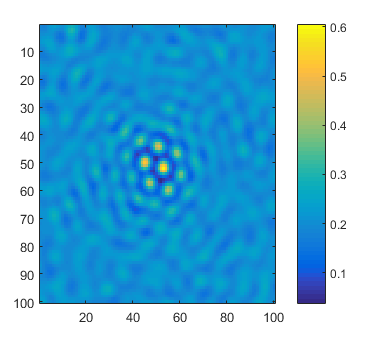
\includegraphics[width=0.5\textwidth]{fig_num/compareTestWavelet1}
}
\subfloat[]
{
    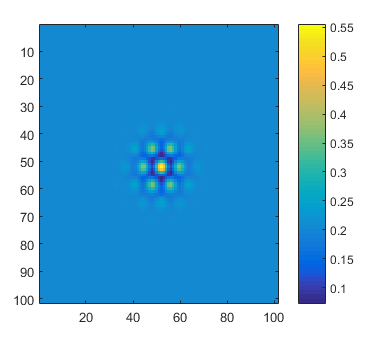
\includegraphics[width=0.5\textwidth]{fig_num/compareTestWavelet2}
}
\caption{(a) Solid grain surrounded by fluctuating liquid, observed in a simulation run with PFC model parameters $n_o=0.207$, $B^x=0.4$, $\Delta B=0.1650$, and $N_a=0.04$. (b) Constructed grain with same model parameters as (a) (except for fluctuations), and with chosen ratios $r_1=0.5$ and $r_2=0.8$. In both figures, the x-axis and y-axis are in number of grid points, and the color bar shows the value of the density field.}\label{fig:num_compareTestWavelet}
\end{figure}

As discussed in section \ref{sec:nuc_cnt_pfc}, we expect that critical nuclei in the PFC model will not depend on only the number of atoms as assumed by CNT. We thus develop a method to efficiently numerically approximate the form of critical nuclei in PFC under the slightly more flexible assumption that both size and order of a grain can vary during the nucleation process. We start by constructing a `test grain', whose density field is given by the predicted density field of a solid bulk in the one-mode approximation from equation \ref{eq:oneMode}, multiplied to a Gaussian envelope centered on one of the peaks. This is written as
%%
\begin{equation}\label{eq:num_testnuc}
n_{test}(x,y) = n_o + \phi \, e^{-(x^2+y^2)/2\sigma^2} \left(\frac{1}{2}\cos\left(\frac{4\pi}{\sqrt[]{3} a}y\right) - \cos\left(\frac{2\pi}{a}+\pi\right)\cos\left(\frac{2\pi}{\sqrt[]{3} a}y\right) \right)
\end{equation}
%%
where the average density of the system $n_o$ and the lattice constant $a$ depend on the model and its chosen parameters as usual, while $\phi$ and $\sigma$ are assumed to be the values that characterize a grain. We set $\phi=r_1 \phi_s$ where $\phi_s$ is the predicted amplitude in the solid bulk, given in equation \ref{eq:freeEnergy_minima}, and $r_1$ is a ratio between 0 and 1. Similarly, set $\sigma=r_2 \, a$ for some ratio $r_2>0$. Effectively, the ratio $r_1$ sets the relative order of the grain with respect to the original liquid and final solid phases, while $r_2$ determines the size of the grain. The ratio $r_1$ can also be heuristically understood as determining the average number of vacancies in the lattice of the forming grain, as it has been argued \cite{berry14} that variations in the amplitude of the PFC model's field can represent vacancy diffusion on diffusive time scales. Figure \ref{fig:num_compareTestWavelet} shows a grain that formed stochastically in a simulated PFC run, as well as a comparable grain constructed with equation \ref{eq:num_testnuc}. The work of formation for any constructed grain can be obtained by subtracting the energy of the unperturbed liquid phase given by equation \ref{eq:freeEnergy_minimized_liquid} from the energy of the grain's system calculated using equation \ref{eq:PFC_energyFunctional}. We note that this approximate grain construction is only expected to be valid for small-radius grains, as large stable solid grains would have a constant amplitude throughout their bulk and a finite interface width. Furthermore, this construction does not account for a variation in \textit{average density} of the grain's interior, as the constructed periodic field would average to $n_o$ over a large enough bulk.

For a given set of PFC model parameters and chosen $r_1$ and $r_2$, we can test whether the constructed grain of equation \ref{eq:num_testnuc} is post-critical or pre-critical by simulating it in a system consisting of the single grain in a much larger amount of liquid phase (grid size given by $L=512$). The fluctuation amplitude is set to zero in this simulation, as the grain is assumed to be the result of a prior fluctuation, and we are interested in the subsequent deterministic evolution of this grain. If after sufficient time steps the grain has grown to fill the system with solid, then it is known to be a post-critical grain, and vice versa. By repeating this test for various $r_1$ and $r_2$ (using a half-interval search method in one of the two variables, for efficiency), we obtain a curve in the space spanned by these two ratios that determines whether a grain with specific $r_1$ and $r_2$ is post-critical. Figure \ref{fig:num_ratioCurve} shows such a curve, which we will refer to as a `critical nucleus curve'. The form of the exactly critical nucleus is thus not unique, as any set of $r_1$ and $r_2$ lying on this curve would give a critical nucleus under the assumptions of the construction of equation \ref{eq:num_testnuc}.

\begin{figure}[!h]
\centering
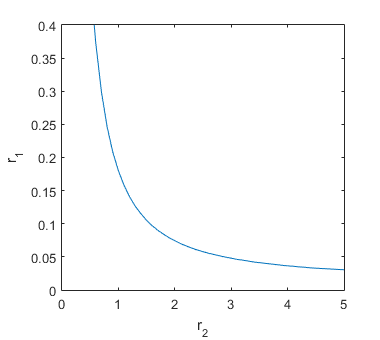
\includegraphics[width=0.6\textwidth]{fig_num/numRatioCurve.png}
\caption{The numerically determined critical nucleus curve for PFC parameters $n_o=0.207$, $B^x=0.4$, and $\Delta B=0.1650$. Choosing a set of ratios $r_1$ and $r_2$ lying above this curve results in a post-critical nucleus, and vice versa.}\label{fig:num_ratioCurve}
\end{figure}

%%%%%%%%%%%%%%%%%%%%%%%%%%%%%%%%%%%%%%%%%%%%%%%%%%%%%%%%%%%%%%%%%%%%%%%%%%%%%%%%%%%%















